\documentclass{beamer}
\usepackage{sdp}

\title{Стек}

\date{24--25 октомври 2017 г.}

\titlegraphicx{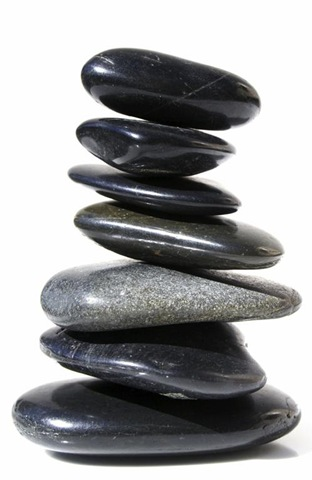
\includegraphics[height=0.25\textheight]{images/stack.jpg}\\
  \imageAttr{Stack of Rocks, Cattle Point, San Juan Island}{Ryan Harvey}{https://flic.kr/p/aojd1Q}{CC BY-SA 2.0}}

\begin{document}

\begin{frame}
  \titlepage
\end{frame}

\section{АТД стек}

\begin{frame}
  \frametitle{АТД: стек}

  Хомогенна линейна структура с организация ``последен влязъл --- пръв излязъл'' (LIFO)\\[1em]
  Операции\\[0.5em]
  \begin{itemize}
  \item \lst{create()} --- създаване на празен стек
  \item \lst{empty()} --- проверка за празнота на стек
  \item \lst{push(x)} --- включване на елемент на стек
  \item \lst{pop()} --- изключване на елемент от стек
  \item \lst{peek()} --- последен елемент на стека
  \end{itemize}
\end{frame}

\begin{frame}
  \frametitle{АТД: стек}

  Свойства на операциите\\[0.5em]
  \begin{itemize}
  \item \lst{create().empty()} = \lst{true}
  \item \lst{s.push(x).empty()} = \lst{false}
  \item \lst{create().peek()}, \lst{create().pop()} --- \alert{грешка}
  \item \lst{s.push(x).peek()} = \tt x
  \item \lst{s.push(x).pop()} = \tt s
  \end{itemize}
\end{frame}

\begin{frame}
  \frametitle{Последователно представяне}
  \newcommand{\pha}{\phantom{$a_0$}}
  %TODO: да се реализира с TikZ и без \phantom
  \begin{center}
    \begin{tabular}{|*{11}{c|}}
      \hline
      \rowcolor{diagramblue}
      $a_0$&$a_1$&$a_2$&\ldots&$a_n$&\alt<1>\pha{$a_{n+1}$}&\pha&\pha&\pha&\pha&\pha\\
      \hline
      \rowcolor{white}
      \multicolumn 4c{}&
      \multicolumn 1c{\onslide<1,3>{\bua}}&
      \multicolumn 1c{\onslide<2 |handout:0>{\bua}}&
      \multicolumn 5c{}\\
      \multicolumn 4c{}&
      \multicolumn 1c{\onslide<1,3>{top}}&
      \multicolumn 1c{\onslide<2 |handout:0>{top}}&
      \multicolumn 5c{}
    \end{tabular}
  \end{center}

  \begin{itemize}
    \item<2-> включване на елемент (push)
    \item<3-> изключване на елемент (pop)
  \end{itemize}
\end{frame}

\begin{frame}
  \frametitle{Свързано представяне}

  %TODO: да се реализира с TikZ
  \begin{center}
    \scriptsize
    \begin{tabular}{cccc@{}c@{}cc}
      \onslide<2-4 |handout:0>{\nextcell{a_{n+1}}}&\nextcell{a_n}&\nextcell{a_{n-1}}&\hspace{1ex}\ldots&$\nextarrow$&\nextcell{a_1}&\nilcell{a_0}\\
      \onslide<2-4 |handout:0>{\bua}&\onslide<1,4-5>{\bua}&\multicolumn 5c{}\\
      \onslide<2-4>{\only<3-4 |handout:0>p\only<3 |handout:0>,\only<2-3 |handout:0>{top}}&\onslide<1,4-5>{top}&\multicolumn 5c{}
    \end{tabular}
  \end{center}

  \begin{itemize}
    \item<2-> включване на елемент (push)
    \item<3-> изключване на елемент (pop)
  \end{itemize}
\end{frame}

\section{Приложения на стек}

\subsection{Пресмятане на израз}

\begin{frame}
  \frametitle{Обратен полски запис}

  %TODO: анимация на обхожданията
  \begin{columns}[t,onlytextwidth]
    \begin{column}{.6\textwidth}
      \begin{itemize}
      \item инфиксен запис:\\
        \lst{(1+2)*(3-4/5)}
      \item префиксен (полски) запис:\\
        \lst{*+12-3/45}
      \item постфиксен (обратен полски) запис\\
        \lst{12+345/-*}
      \end{itemize}
    \end{column}

    \begin{column}{0.4\textwidth}
      \begin{center}
        \begin{forest} for tree={circle,draw,fill=diagramblue}
          [\tt* [\tt+ [\tt1] [\tt2]] [\tt- [\tt3] [\tt/ [\tt4] [\tt5]]]]
        \end{forest}
      \end{center}
    \end{column}
  \end{columns}
\end{frame}

\begin{frame}
  \frametitle{Пресмятане на израз в обратен полски запис}

  %TODO: да се реализира с TikZ
  \begin{center}
    \begin{tabular}{|p{20ex}p{25ex}@{}m{0pt}@{}}
      \hline
      \cellcolor{diagramblue}&\multicolumn 1{c|}{\cellcolor{diagramblue}обратен полски запис}&\\[3em]
      \cline{2-3}
      \multicolumn 1{|c|}{\cellcolor{diagramblue}резултати}&\multicolumn 1c{}&\\[7em]
      \cline{1-1}
    \end{tabular}
  \end{center}
\end{frame}

\begin{frame}<handout:0>
  \frametitle{Пример: Пресмятане на израз в обратен полски запис}

  % TODO: да се реализира с TikZ
  % TODO: да се опише алгоритъма в текстов вид
  \begin{center}
    \begin{tabular}{|p{20ex}p{15ex}@{}m{0pt}@{}}
      \hline
      \cellcolor{diagramblue}&\multicolumn 1{c|}{\cellcolor{diagramblue}
      \tt{
      \onslide<-+>1%
      \onslide<-+>2%
      \onslide<-+>+%
      \onslide<-+>3%
      \onslide<-+>4%
      \onslide<-+>5%
      \onslide<-+>/%
      \onslide<-+>-%
      \onslide<-+>*%
      \onslide<-+>\phantom
      }}
      &\\[3em]
      \cline{2-3}
      \multicolumn 1{|c|}{\cellcolor{diagramblue}
      \begin{tabular}{c}
        \only<10>{\\\tt{6.6}}%
        \only<9>{\\\tt{2.2}}%
        \only<8>{\\\tt{0.8}}%
        \only<7>{\\\tt 5}%
        \only<6-7>{\\\tt 4}%
        \only<5-8>{\\\tt 3}%
        \only<4-9>{\\\tt 3}%
        \only<3>{\\\tt 2}%
        \only<2-3>{\\\tt 1}%
      \end{tabular}
      }&\multicolumn 1c{}&\\[7em]
      \cline{1-1}
    \end{tabular}
  \end{center}
\end{frame}

% TODO: общ слайд за преобразуване в обратен полски запис

\begin{frame}<handout:0>
  \frametitle{Пример: Преобразуване в обратен полски запис}

  % TODO: да се реализира с TiKZ
  % TODO: да се опише алгоритъма в текстов вид
  \begin{center}
    \begin{tabular}{p{25ex}p{20ex}p{20ex}@{}m{0pt}@{}}
      \hline
      \multicolumn 1{|c}{\cellcolor{diagramblue}%
      \tt{%
      \only<3->1%
      \only<5->2%
      \only<8->+%
      \only<12->3%
      \only<14->4%
      \only<16->5%
      \only<19->/%
      \only<20->-%
      \only<22->*%
      }}&\cellcolor{diagramblue}&\multicolumn 1{c|}{\cellcolor{diagramblue}%
      \tt{%
      \onslide<-1>(%
      \onslide<-2>1%
      \onslide<-3>+%
      \onslide<-4>2%
      \onslide<-5>)%
      \onslide<-9>*%
      \onslide<-10>(%
      \onslide<-11>3%
      \onslide<-12>-%
      \onslide<-13>4%
      \onslide<-14>/%
      \onslide<-15>5%
      \onslide<-16>)%
      \onslide<-22>\phantom
      }}&\\[3em]
      \cline{1-1} \cline{3-3}
      \multicolumn 1{p{20ex}}{}&\multicolumn 1{|c|}{\cellcolor{diagramblue}%
      \begin{tabular}{c}
      \only<17>{\\\tt)}%
      \only<15-18>{\\\tt/}%
      \only<13-19>{\\\tt-}%
      \only<11-20>{\\\tt(}%
      \only<10-21>{\\\tt*}%
      \only<6>{\\\tt)}%
      \only<4-7>{\\\tt+}%
      \only<2-8>{\\\tt(}%
      \end{tabular}
      }&\multicolumn 1c{}&\\[7em]
      \cline{2-2}
    \end{tabular}
  \end{center}
\end{frame}

% TODO: Слайд за проблема с приоритетите

\begin{frame}<handout:0>
  \frametitle{Пример 2: Преобразуване в обратен полски запис}

  % TODO: да се реализира с TiKZ
  \begin{center}
    \begin{tabular}{p{25ex}p{20ex}p{20ex}@{}m{0pt}@{}}
      \hline
      \multicolumn 1{|c}{\cellcolor{diagramblue}%
      \tt{%
      \only<3->1%
      \only<5->2%
      \only<8->+%
      \only<12->3%
      \only<14->4%
      \only<15->/%
      \only<16->5%
      \only<19->-%
      \only<21->*%
      }}&\cellcolor{diagramblue}&\multicolumn 1{c|}{\cellcolor{diagramblue}%
      \tt{%
      \onslide<-1>(%
      \onslide<-2>1%
      \onslide<-3>+%
      \onslide<-4>2%
      \onslide<-5>)%
      \onslide<-9>*%
      \onslide<-10>(%
      \onslide<-11>3%
      \onslide<-12>/%
      \onslide<-13>4%
      \onslide<-14>-%
      \onslide<-15>5%
      \onslide<-16>)%
      \onslide<-21>\phantom
      }}&\\[3em]
      \cline{1-1} \cline{3-3}
      \multicolumn 1{p{20ex}}{}&\multicolumn 1{|c|}{\cellcolor{diagramblue}%
      \begin{tabular}{c}
      \only<17>{\\\tt)}%
      \only<15-18>{\\\tt-}%
      \only<13-14>{\\\tt/}%
      \only<11-19>{\\\tt(}%
      \only<10-20>{\\\tt*}%
      \only<6>{\\\tt)}%
      \only<4-7>{\\\tt+}%
      \only<2-8>{\\\tt(}%
      \end{tabular}
      }&\multicolumn 1c{}&\\[7em]
      \cline{2-2}
    \end{tabular}
  \end{center}
\end{frame}


\begin{frame}
  \frametitle{Директно пресмятане на израз}

  % TODO: да се реализира с TiKZ  
  \begin{center}
    \begin{tabular}{|p{20ex}p{5ex}p{20ex}p{20ex}@{}m{0pt}@{}}
      \hline
      \cellcolor{diagramblue}&\cellcolor{diagramblue}&\cellcolor{diagramblue}&\multicolumn 1{c|}{\cellcolor{diagramblue}инфиксен запис}&\\[3em]
      \cline{2-2} \cline{4-4}
      \multicolumn 1{|c|}{\cellcolor{diagramblue}резултати}&\multicolumn 1c{}&\multicolumn 1{|c|}{\cellcolor{diagramblue}операции}&\multicolumn 1c{}&\\[7em]
      \cline{1-1} \cline{3-3}
    \end{tabular}
  \end{center}
\end{frame}

\begin{frame}<handout:0>
  \frametitle{Пример: Директно пресмятане на израз}

  % TODO: да се реализира с TiKZ
  % TODO: да се опише алгоритъма в текстов вид
  \begin{center}
    \begin{tabular}{|p{20ex}p{5ex}p{20ex}p{20ex}@{}m{0pt}@{}}
      \hline
      \cellcolor{diagramblue}&\cellcolor{diagramblue}&\cellcolor{diagramblue}&\multicolumn 1{c|}{\cellcolor{diagramblue}\tt{%
      \onslide<-1>(%
      \onslide<-2>1%
      \onslide<-3>+%
      \onslide<-4>2%
      \onslide<-5>)%
      \onslide<-9>*%
      \onslide<-10>(%
      \onslide<-11>3%
      \onslide<-12>-%
      \onslide<-13>4%
      \onslide<-14>/%
      \onslide<-15>5%
      \onslide<-16>)%
      \phantom !%
      \onslide<-22>\phantom
      }}&\\[3em]
      \cline{2-2} \cline{4-4}
      \multicolumn 1{|c|}{\cellcolor{diagramblue}
      \begin{tabular}{c}
        \only<22>{\\\tt{6.6}}%
        \only<20-21>{\\\tt{2.2}}%
        \only<19>{\\\tt{0.8}}%
        \only<16-18>{\\\tt5}%
        \only<14-18>{\\\tt4}%
        \only<12-19>{\\\tt3}%
        \only<8-21>{\\\tt3}%
        \only<5-7>{\\\tt2}%
        \only<3-7>{\\\tt1}%
      \end{tabular}
      }&\multicolumn 1c{}&\multicolumn 1{|c|}{\cellcolor{diagramblue}
      \begin{tabular}{c}
      \only<17>{\\\tt)}%
      \only<15-18>{\\\tt/}%
      \only<13-19>{\\\tt-}%
      \only<11-20>{\\\tt(}%
      \only<10-21>{\\\tt*}%
      \only<6>{\\\tt)}%
      \only<4-7>{\\\tt+}%
      \only<2-8>{\\\tt(}%
      \end{tabular}
      }&\multicolumn 1c{}&\\[7em]
      \cline{1-1} \cline{3-3}
    \end{tabular}
  \end{center}
\end{frame}

%TODO: слайд за поточна обработка

\subsection{Симулиране на рекурсия}

\begin{frame}
  \frametitle{Симулиране на рекурсия}

  \begin{itemize}
  \item Стекова рамка
    \begin{itemize}
    \item при извикване на функция
    \item при рекурсия
    \end{itemize}
  \item Стек вместо стекова рамка
  \item Пример: ход на коня
  \end{itemize}
\end{frame}

\begin{frame}
  \frametitle{Пример: ход на коня}

  % TODO: да се нарисува с TikZ
  \begin{columns}[t,onlytextwidth]
    \begin{column}{.5\textwidth}
      \begin{chessboard}4{1ex}
        \hline\bks1&\ws&\bks9&\ws&\\[1ex]
        \hline\bks{10,11}&\ws&\bks2&\bks5&\\[1ex]
        \hline\bks3&\safetemporal6\ws\bk{\alt<8>\bk\wk}&\ws&\ws&\\[1ex]
        \hline\ws&\ws&\bks4&\bks7&\\[1ex]
        \hline
      \end{chessboard}
    \end{column}

    % TODO: различен цвят за коня на обратния ход
    \begin{column}{.5\textwidth}
      \begin{tabular}{|c|cc}
        \cline{1-1}
        \\\cline{1-1}
        \\\cline{1-1}\onslide<10->{(1,0)}
        \\\cline{1-1}\onslide<7->{\safetemporal8{(3,3)}{}{(0,2)}}
        \\\cline{1-1}\onslide<6->{(2,1)}&\gc{11-}{(0,1)}
        \\\cline{1-1}\onslide<5->{(1,3)}&\gc{11-}{(1,1)}
        \\\cline{1-1}\onslide<4->{(3,2)}&\gc{11-}{(0,1)}
        \\\cline{1-1}\onslide<3->{(2,0)}&\gc{11-}{(3,1)}&\gc{11-}{(3,3)}
        \\\cline{1-1}\onslide<2->{(1,2)}&\gc{11-}{(2,1)}
        \\\cline{1-1}\onslide<1->{(0,0)}
        \\\cline{1-1}
      \end{tabular}
    \end{column}
  \end{columns}
\end{frame}

\section{STL}

\begin{frame}
  \frametitle{\lst{std::stack<T>}}

  \begin{itemize}
  \item \lst{stack()} --- създаване на празен стек
  \item \lst{empty()} --- проверка за празнота на стек
  \item \lst{push(x)} --- включване на елемент на стек
  \item \lst{pop()} --- изключване на елемент от стек
  \item \lst{top()} --- последен елемент на стека
  \item \lst{size()} --- дължина на стека
  \item \lst{==,!=,<,>,<=,>=} --- лексикорафско сравнение на два стека
  \end{itemize}
\end{frame}

\end{document}
